\documentclass[12pt]{article}
\usepackage{pgf, tikz}
\usepackage{amsmath, amsfonts, amssymb, graphicx}
\usepackage{float}
\usepackage{subfig}
\usepackage[utf8]{inputenc}
\usepackage[spanish]{babel}
\usepackage{amsthm}
\usepackage{caption}

\setlength{\textheight}{23cm} \setlength{\evensidemargin}{0cm}
\setlength{\oddsidemargin}{-.5cm} \setlength{\topmargin}{-3cm}
\setlength{\textwidth}{17.5cm} \setlength{\parskip}{.2cm}


%opening

\begin{document}
	\begin{picture}(80, 80)
	\put(170,0){\hbox{
\includegraphics[scale=0.6]{cimat_logo.png}}}
	\end{picture}
	
	\begin{center}
		\begin{huge}
			Centro de Investigación en Matemáticas, A.C.
		\end{huge}
	\end{center}

	\begin{center}
		\begin{large}
			Descripción tarea 12 - Métodos numéricos
		\end{large}
	\end{center}
	
	\begin{center}
		\textbf{Erick Salvador Alvarez Valencia}
	\end{center}

	\begin{center}
		18 de Noviembre de 2017
	\end{center}



%\maketitle

%\tableofcontents

\section{Introducción}
En el presente reporte se describirán los resultados obtenidos del método trapezoidal que se utilizó para resolver un problema de valor inicial (PVI) con una ecuación diferencial de segundo orden. Se describirá un poco la descripción del método utilizado para resolver el PVI así como ejemplos de los resultados obtenidos.

\section{Descripción}
El método consistió en realizar una discretización en un intervalo cerrado y convertir el PVI en un sistema de matricial, posteriormente se aplicó el método del trapecio en el mismo y se obtuvo un método implícito en donde se debió despejar el valor de $y_{i+1}$ con lo que se llegó a un sistema de ecuaciones que es resoluble con algún método ya sea directo o iterativo, para el presente se utilizó el método de factorización LU.\\

A continuación se muestra el PVI:

$$y'' = -y + xy' - 2x \cos x$$

Con $y(0) = 0$ y $y'(0) = 3$.

La solución analítica de dicho problema es: $y(x) = x + 2 \sin x$.

El sistema de ecuaciones al cual se llegó con el método del trapecio se muestra en las hojas adjuntas al programa.

\section{Ejemplo de ejecución}
El programa se ejecutó con diferentes tamaños de la discretización, todos dentro del intervalo $[0, 5]$ y dentro de las ejecuciones se registró el error absoluto promedio y el error absoluto máximo, estos en comparación con el resultado de la solución analítica. De la misma forma se imprimió el último valor numérico calculado y el valor analítico en ese mismo $x_i$. A continuación se muestran dos de los resultados obtenidos con diferentes valores de $n$.

\begin{figure}[H]
	\centering
	\subfloat[][Figura 1. Resultados del programa, n = 400.]{
		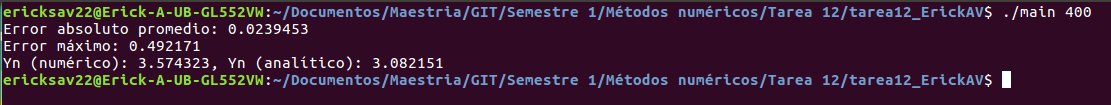
\includegraphics[scale=0.4]{E1.png}
	}\hfill
\end{figure}

\begin{figure}[H]
	\centering
	\subfloat[][Figura 2. Resultados del programa, n = 4000.]{
		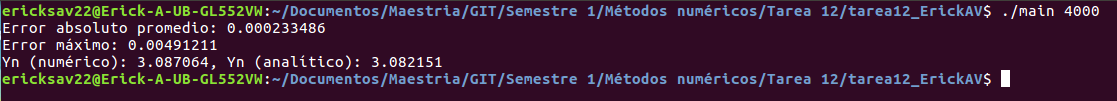
\includegraphics[scale=0.4]{E2.png}
	}\hfill
\end{figure}

Se puede ver en la Figura 2. que pese a que aumentó mucho el número de valores en la discretización, la solución tuvo una notable mejoría en comparación con la analítica, así mismo los errores se hicieron más pequeños.

\section{Compilación y ejecución}
\textbf{Para compilar:} En la carpeta encontraremos los archivos $.c$ y $.h$ con los que se podrá compilar el ejecutable. De la misma forma, en conjunto con los archivos anteriores, también podremos encontrar un Makefile para, en caso de encontrarse en linux, compilar de manera sencilla.

\begin{enumerate}
	\item \textbf{Compilar usando Makefile:} En la terminal, nos colocamos en el directorio donde se encuentre el programa, y ejecutamos el comando $make$, automáticamente se realizará la compilación y se generará el ejecutable. El Makefile también contiene el comando $make\ help$ el cual mostrará todas las opciones disponibles.
	\item \textbf{Compilar directamente:} De la misma forma, podemos compilar directamente usando los siguientes comandos (en terminal):
	\begin{itemize}
		\item gcc -c main.c -o obj/main.o
		\item gcc -c memo.c -o obj/memo.o
		\item gcc -c matriz\_vector.c -o obj/matriz\_vector.o
		\item gcc -c met\_num.c -o obj/met\_num.o
		\item gcc -o main obj/main.o obj/memo.o obj/matriz\_vector.o obj/met\_num.o\ -lm
	\end{itemize}
\end{enumerate}

\textbf{Para ejecutar:} Únicamente debemos de usar el comando $./main$ para ejecutar el programa en consola, este recibe el siguiente argumento:
\begin{itemize}
	\item \textbf{Un número entero:} El tamaño de la discretización.
\end{itemize}

El programa ejecutará el método trapezoidal para el PVI mostrado anteriormente dentro del intervalo [0, 5]. Se mostrará como resultado el error absoluto promedio y el error absoluto máximo, así como el último valor $y_n$ y el valor de la solución analítica.\\

\textbf{Ejemplo de ejecución:} ./main 400\\

\end{document}
